\documentclass[14pt,a4paper]{extarticle}
% =============================================================
% preamble.tex — общая преамбула отчётов по дисциплине
% «Стили и методы программирования. Часть 2»
% Оформление по СТП БГУИР 01-2024; сборка XeTeX (tectonic)
% =============================================================

% Encoding and language
\usepackage{fontspec}
\usepackage[russian]{babel}

% Times New Roman font
\setmainfont{Times New Roman}
\setmonofont{Menlo}[Scale=0.85]

% Page geometry: STP 2.1.1
\usepackage{geometry}
\geometry{left=30mm, right=15mm, top=20mm, bottom=20mm}

% Line spacing: STP 2.1.1
\usepackage{setspace}
\singlespacing

% Allow TeX a bit more flexibility to avoid overflow
\pretolerance=1000
\tolerance=2000
\emergencystretch=3em

% Paragraph indent
\usepackage{indentfirst}
\setlength{\parindent}{1.25cm}

% Page numbers
\usepackage{fancyhdr}
\pagestyle{fancy}
\fancyhf{}
\fancyfoot[R]{\thepage}
\renewcommand{\headrulewidth}{0pt}
\fancypagestyle{plain}{%
  \fancyhf{}%
  \fancyfoot[R]{\thepage}%
  \renewcommand{\headrulewidth}{0pt}%
}

% Math
\usepackage{amsmath,amssymb}

% Graphics
\usepackage{graphicx}
\usepackage{float}
\usepackage{xcolor}

% Tables
\usepackage{booktabs}
\usepackage{tabularx}
\usepackage{multirow}
\usepackage{longtable}

% Captions
\usepackage{caption}
\captionsetup[figure]{
  labelsep=endash,
  justification=centering,
  font={normalsize},
  name=Рисунок
}
\captionsetup[table]{
  labelsep=endash,
  justification=raggedright,
  singlelinecheck=false,
  font={normalsize},
  name=Таблица
}

% Section formatting
\usepackage{titlesec}
% Каждый раздел с новой страницы. \newpage внутри \titleformat срабатывает
% после записи в оглавление и сбивает номера страниц, поэтому \clearpage
% ставится перед самой командой \section.
\usepackage{etoolbox}
\pretocmd{\section}{\clearpage}{}{}
\titleformat{\section}
  {\normalfont\fontsize{14}{18}\selectfont\bfseries}
  {\thesection}{0.5em}{\MakeUppercase}
\titlespacing*{\section}{1.25cm}{0pt}{14pt}

\titleformat{\subsection}
  {\normalfont\fontsize{14}{18}\selectfont\bfseries}
  {\thesubsection}{0.5em}{}
\titlespacing*{\subsection}{1.25cm}{14pt}{14pt}

\titleformat{\subsubsection}
  {\normalfont\fontsize{14}{18}\selectfont\bfseries}
  {\thesubsubsection}{0.5em}{}
\titlespacing*{\subsubsection}{1.25cm}{14pt}{14pt}

% Unnumbered sections
\newcommand{\sectioncenter}[1]{%
  \newpage
  \phantomsection
  \addcontentsline{toc}{section}{#1}
  \begin{center}
    \textbf{\MakeUppercase{#1}}
  \end{center}
  \vspace{14pt}
}

% Table of contents formatting
\usepackage{tocloft}
\renewcommand{\cftsecfont}{\normalfont}
\renewcommand{\cftsecpagefont}{\normalfont}
\renewcommand{\cftsubsecfont}{\normalfont}
\renewcommand{\cftsubsecpagefont}{\normalfont}
\renewcommand{\cftsecleader}{\cftdotfill{\cftdotsep}}
\renewcommand{\cftdotsep}{1}
% babel переопределяет \contentsname при \begin{document}, поэтому через captionsrussian
\addto\captionsrussian{\renewcommand{\contentsname}{СОДЕРЖАНИЕ}}
\renewcommand{\cfttoctitlefont}{\hfill\normalfont\bfseries}
\renewcommand{\cftaftertoctitle}{\hfill}

% Lists
\usepackage{enumitem}
\setlist[itemize]{noitemsep, topsep=0pt, leftmargin=1.25cm, label=--}
\setlist[enumerate]{noitemsep, topsep=0pt, leftmargin=1.25cm}

% Code listings: fvextra корректно работает с Unicode под XeTeX
% (listings переставляет символы «», —, № в комментариях)
\usepackage{fvextra}
\fvset{
  frame=single,
  fontsize=\small,
  numbers=left,
  numbersep=6pt,
  breaklines=true,
}
\newcommand{\code}[1]{\texttt{#1}}

% Hyperlinks
\usepackage{hyperref}
\hypersetup{
  colorlinks=true,
  linkcolor=black,
  urlcolor=blue,
  citecolor=black,
}

% Number figures and tables within sections
\numberwithin{figure}{section}
\numberwithin{table}{section}
\numberwithin{equation}{section}

% Титульный лист: \makelabtitle{номер}{тема}{дата}
\newcommand{\makelabtitle}[3]{%
  \begin{titlepage}
  \thispagestyle{empty}
  \begin{center}

  МИНИСТЕРСТВО ОБРАЗОВАНИЯ РЕСПУБЛИКИ БЕЛАРУСЬ

  \vspace{0.5em}

  Учреждение образования

  \vspace{0.5em}

  \textbf{<<Белорусский государственный университет информатики и радиоэлектроники>>}

  \vspace{2em}

  Факультет компьютерных систем и сетей

  \vspace{0.5em}

  Кафедра программного обеспечения информационных технологий

  \end{center}

  \vspace{3em}

  \begin{center}
  \textbf{ОТЧЕТ}

  \vspace{0.5em}

  по практической работе №#1

  \vspace{0.5em}

  по дисциплине

  \vspace{0.5em}

  <<Стили и методы программирования. Часть 2 (МДН)>>

  \vspace{0.5em}

  на тему

  \vspace{0.5em}

  <<#2>>
  \end{center}

  \vspace{5em}

  \begin{flushright}
  \begin{minipage}{0.5\textwidth}
  \textbf{Выполнил:}\\
  Лебедевич Артем Владимирович\\
  магистрант 2 курса группы 556301

  \vspace{0.6em}

  \textbf{Преподаватель:}\\
  Парамонов Антон Иванович\\
  кандидат технических наук\\
  доцент

  \vspace{0.6em}

  \textbf{Дата:} #3
  \end{minipage}
  \end{flushright}

  \vfill

  \begin{center}
  Минск, 2026~г.
  \end{center}

  \end{titlepage}
}

\graphicspath{{figures/}}

\begin{document}

\makelabtitle{2}{Разработка логических программ на языке Prolog для работы с базами знаний и решения задач поиска}{11.10.2026}

\tableofcontents

\newpage

\section{Цель работы}

Изучить базовый синтаксис и семантику языка Prolog, освоить методы создания и модификации динамических баз фактов и правил, научиться решать задачи логического вывода и поиска с ограничениями.

\section{Используемое ПО}

Версия интерпретатора и параметры программной среды приведены в таблице~\ref{tab:env}; результат запроса версии показан на рисунке~\ref{fig:env}.

\begin{table}[H]
\caption{Программная среда}
\label{tab:env}
\centering
\begin{tabularx}{\textwidth}{@{}lX@{}}
\toprule
Параметр & Значение \\
\midrule
Интерпретатор Prolog & SWI-Prolog 10.0.2 (threaded, 64 bits), сборка \code{arm64-darwin} \\
Способ установки & менеджер пакетов Homebrew, формула \code{swi-prolog} \\
Операционная система & macOS 26.6.2 (сборка 25G83) \\
Аппаратная платформа & Apple M4 Pro, архитектура arm64 \\
Интерпретатор & \code{/opt/homebrew/bin/swipl}, консольный top-level в терминале zsh \\
Редактор & Visual Studio Code \\
Кодировка исходных файлов & UTF-8; атомы и имена предикатов записаны кириллицей \\
Рабочая директория & \code{\textasciitilde/Projects/prolog/lab\_02} \\
\bottomrule
\end{tabularx}
\end{table}

\begin{figure}[H]
\centering
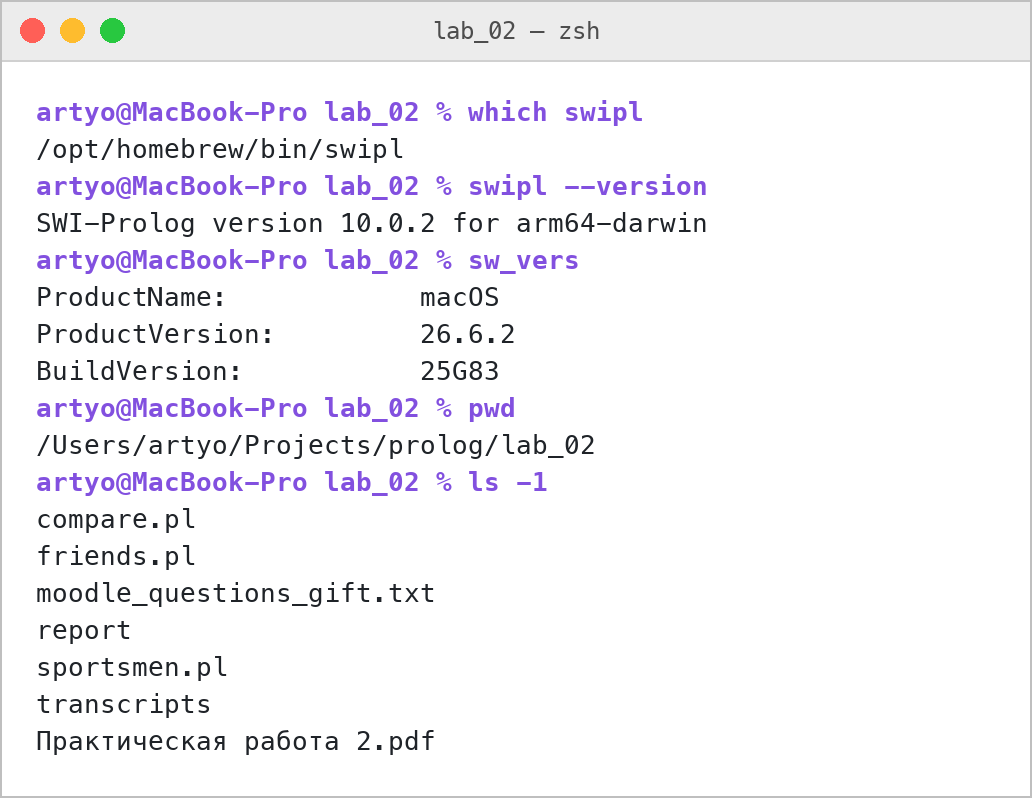
\includegraphics[width=0.8\textwidth]{fig01_env.png}
\caption{Версия интерпретатора, ОС и содержимое рабочей директории проекта}
\label{fig:env}
\end{figure}

\textbf{Обоснование выбора.} Использован тот же SWI-Prolog, что и в практической работе~1: он соответствует стандарту ISO, содержит нужные для работы встроенные средства (динамические предикаты \code{assertz/retract}, ввод строк, \code{findall/3}, \code{permutation/2}) и корректно работает с кириллицей в атомах, что позволяет записывать базы знаний варианта в том виде, в котором они даны в задании.

\section{Ход выполнения работы}

\subsection{Создание проекта}

Новый проект~--- директория \code{lab\_02} внутри репозитория \code{prolog}. Каждое задание оформлено отдельным файлом с программой (таблица~\ref{tab:files}); интерпретатор запускается из этой директории, поэтому файлы загружаются по короткому имени: \code{swipl compare.pl} либо \code{?- [compare].}

\begin{table}[H]
\caption{Состав проекта}
\label{tab:files}
\centering
\begin{tabularx}{\textwidth}{@{}llX@{}}
\toprule
Задание & Файл & Содержание \\
\midrule
2 & \code{compare.pl} & динамическая база отношений «больше», ввод с консоли, поиск наибольшего и наименьшего объекта \\
3 & \code{friends.pl} & база знаний «Друзья» (вариант~3) и ответы на её вопросы \\
4 & \code{sportsmen.pl} & логическая задача про спортсменов (вариант~3) \\
\bottomrule
\end{tabularx}
\end{table}

\subsection{Задание 2: динамическая база фактов об отношении «больше»}

\textbf{Постановка.} С консоли вводятся отношения между объектами, например: <<яблоко больше сливы>>, <<авокадо меньше папайи>>. Число объектов заранее неизвестно, ввод продолжается до заданного символа. По введённым фактам нужно определить самый большой и самый маленький объекты.

\textbf{Решение.} Программа \code{lab\_02/compare.pl} приведена ниже. Отношение вводится строкой вида \code{A > B} (A больше B) или \code{A < B} (A меньше B); допустимы и слова <<больше>>, <<меньше>>. Символом остановки служит \code{\#}, он задан фактом \code{stop\_symbol/1}.

\VerbatimInput{../compare.pl}

\textbf{Основная логика.}

\begin{enumerate}
\item \textbf{Динамическая база.} Директивы \code{:- dynamic} объявляют предикаты \code{bigger/2} (факт <<X больше Y>>) и \code{object/1} (объект встретился во вводе) изменяемыми во время работы. Факты добавляются вызовом \code{assertz/1} в порядке ввода; в начале \code{start/0} база очищается через \code{retractall/1}, поэтому программу можно запускать повторно.
\item \textbf{Ввод.} Предикат \code{read\_relations/1} рекурсивно читает строки \code{read\_line\_to\_string/2} до символа остановки или конца ввода (Ctrl+D). Рекурсия хвостовая, число строк не ограничено. Стандартное приглашение <<\code{|: }>> убрано вызовом \code{prompt/2}, вместо него печатается своё, поэтому \code{flush\_output/0} вызывается до чтения. Строка нормализуется (\code{normalize\_space/2}), приводится к нижнему регистру и разбивается \code{split\_string/4} на три части: два объекта и знак.
\item \textbf{Контроль данных.} Предикат \code{add\_relation/2} отклоняет отношение объекта к самому себе и факт, противоречащий уже известным (если $Y$ больше $X$ прямо или по цепочке), а уже выводимый факт не дублирует. Без этой проверки цикл (<<a больше b>>, <<b больше a>>) привёл бы к бесконечной рекурсии в \code{greater/2}. Строка неверного формата сообщается и пропускается.
\item \textbf{Правила вывода.} \code{greater/2}~--- транзитивное замыкание: базовый случай~--- прямой факт \code{bigger}, рекурсивный шаг~--- цепочка через промежуточный объект. Правило \code{largest(X)} истинно для объекта, которого не превосходит ни один другой (\code{\textbackslash+ bigger(\_, X)}); \code{smallest(X)}~--- для объекта, который не больше никакого.
\item \textbf{Ответ.} \code{report/0} собирает решения \code{largest/1} и \code{smallest/1} в списки через \code{findall/3}. Если в списке один объект, он и есть ответ; если несколько, единого наибольшего (наименьшего) нет~--- объекты принадлежат разным цепочкам и между собой несравнимы, о чём выводится сообщение.
\end{enumerate}

\textbf{Результаты.} На рисунке~\ref{fig:compare-task} введён пример из задания: <<яблоко больше сливы, авокадо больше сливы, но меньше папайи, дуриан больше папайи, вишня меньше сливы>>. Принятые отношения нормализованы к виду <<больше>> (<<авокадо меньше папайи>> $\to$ <<папайя больше авокадо>>). Команда \code{listing(bigger/2)} показывает, что база действительно построена во время работы программы, а \code{greater(дуриан, вишня)} выводит факт, которого в базе нет: дуриан $>$ папайя $>$ авокадо $>$ слива $>$ вишня.

Самый маленький объект~--- вишня. Единого самого большого нет: цепочка \code{дуриан > папайя > авокадо > слива > вишня} и отношение \code{яблоко > слива} не позволяют сравнить яблоко с дурианом, поэтому программа выдаёт оба максимальных объекта. Ответ <<дуриан>> появляется, если добавить недостающее условие <<яблоко меньше дуриана>> (рисунок~\ref{fig:compare-unique}).

\begin{figure}[H]
\centering
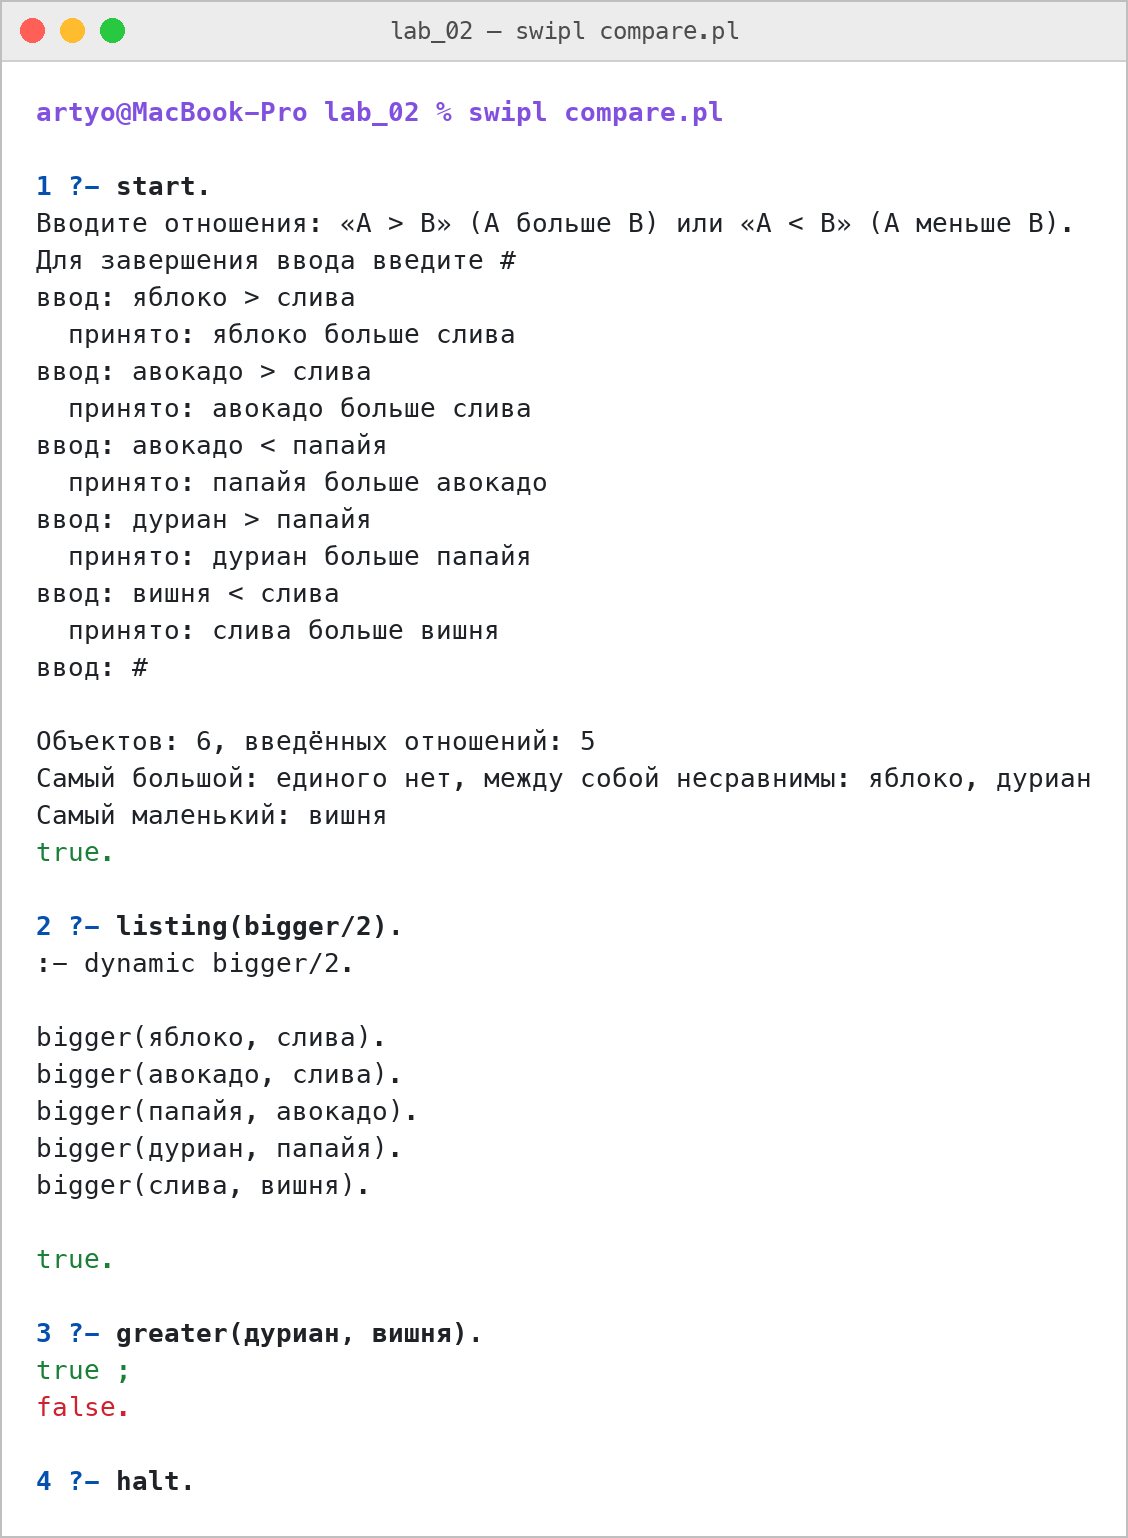
\includegraphics[width=0.62\textwidth]{fig02_compare_task.png}
\caption{Пример из задания: ввод отношений, ответ, содержимое динамической базы}
\label{fig:compare-task}
\end{figure}

\begin{figure}[H]
\centering
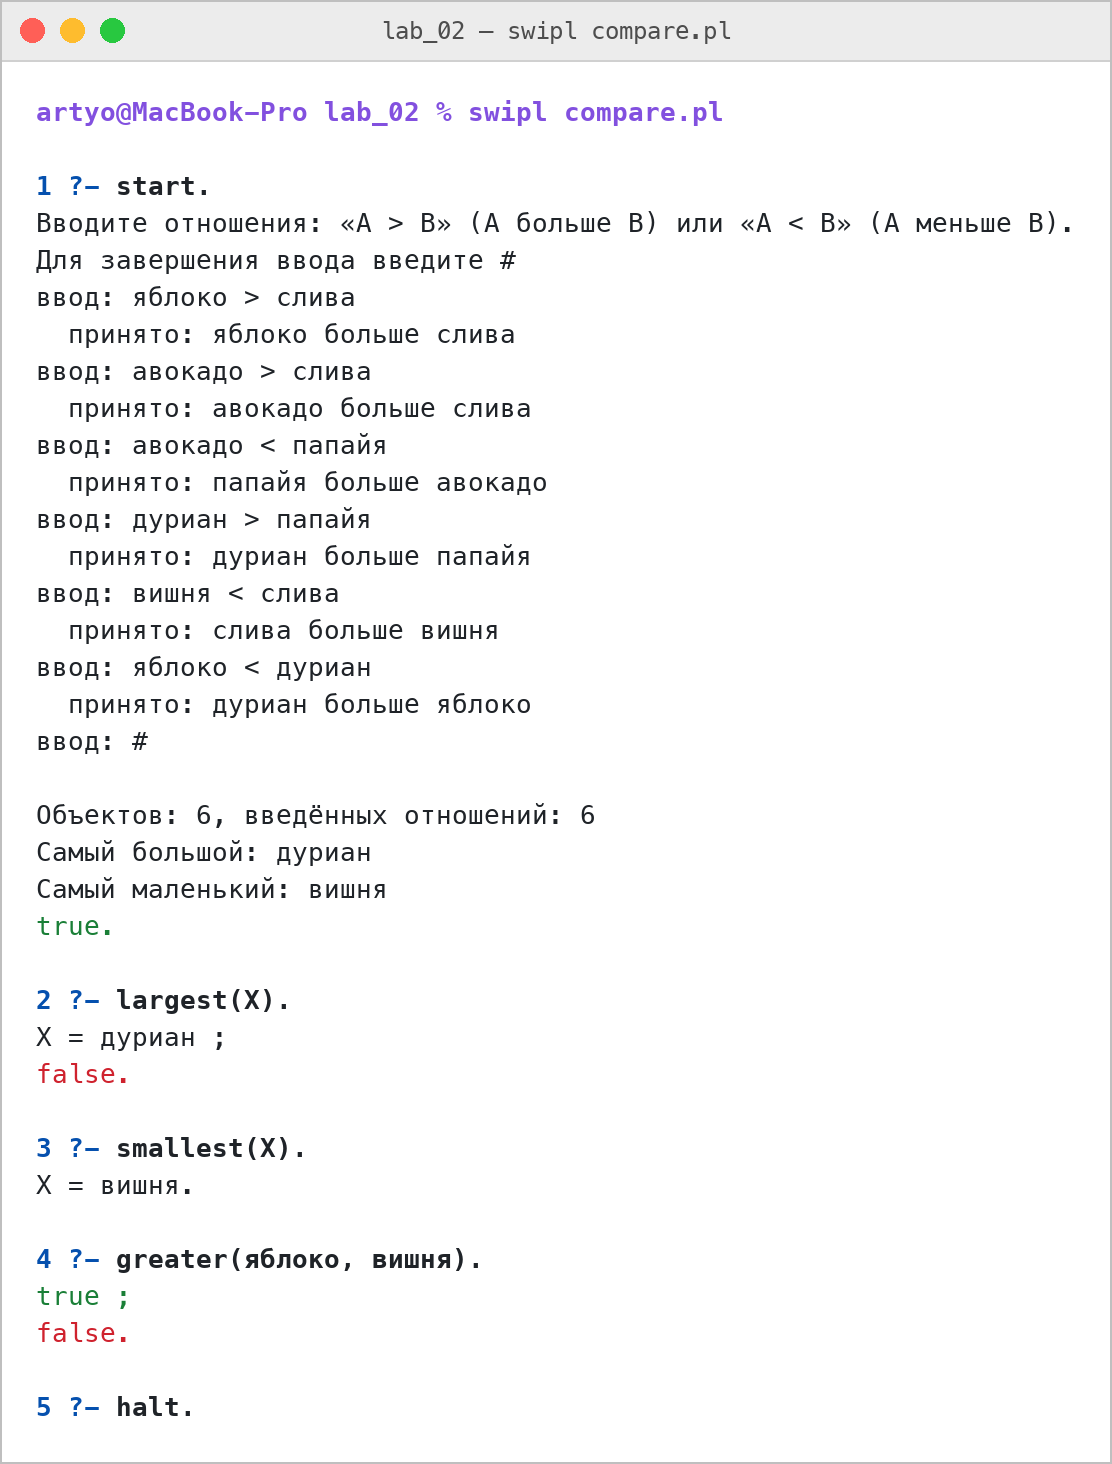
\includegraphics[width=0.62\textwidth]{fig03_compare_unique.png}
\caption{Тот же ввод с дополнительным условием <<яблоко меньше дуриана>>}
\label{fig:compare-unique}
\end{figure}

Работа с некорректными данными показана на рисунке~\ref{fig:compare-errors}: противоречие, сравнение объекта с самим собой, неизвестный знак, пустая строка, повтор и факт, уже выводимый из известных.

\begin{figure}[H]
\centering
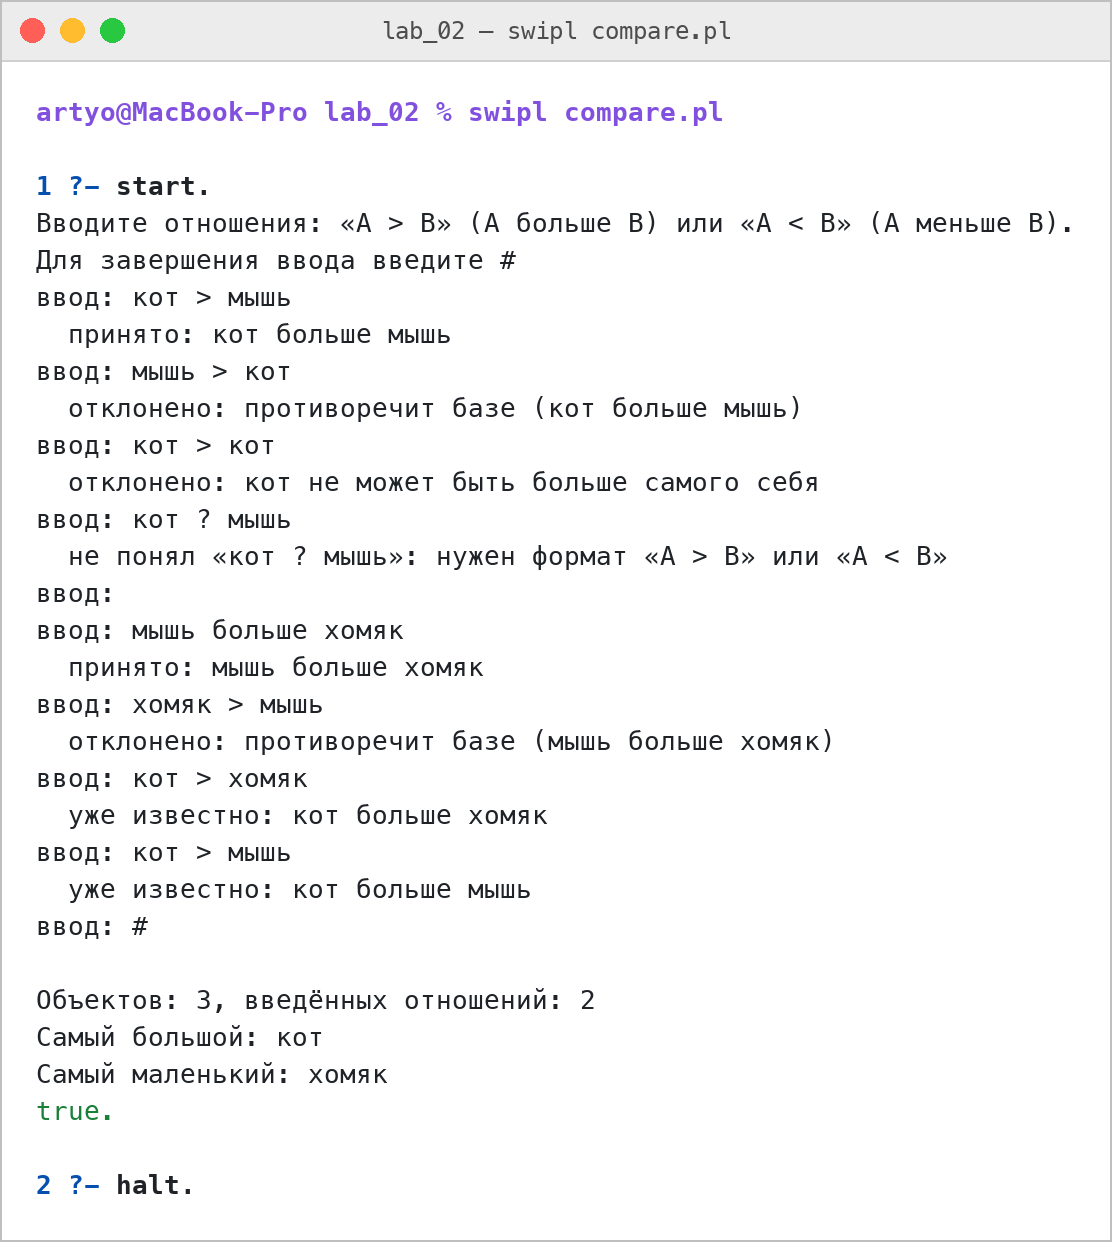
\includegraphics[width=0.7\textwidth]{fig04_compare_errors.png}
\caption{Обработка некорректного и избыточного ввода}
\label{fig:compare-errors}
\end{figure}

\subsection{Задание 3: база знаний <<Друзья>> (вариант 3)}

\textbf{Постановка.} Написать программу для базы знаний <<Друзья>> и ответить на вопросы: кто родился в 1988 году; кто родился в мае; у кого хобби книги; какое хобби у Маши; у кого хобби и кино, и спорт; вывести список фамилий и имён всех друзей.

\textbf{Решение.} Программа \code{lab\_02/friends.pl}. Факты \code{день\_рождения/5} и \code{хобби/3} записаны в точности как в задании. Поверх них добавлены правила: \code{друг/2} (каждый друг указан днём рождения), \code{родился\_в\_году/3}, \code{родился\_в\_месяце/3} и \code{увлекается\_обоими/4}. Предикат \code{ответы/0} печатает ответы на все вопросы; вспомогательный \code{вывести/3} собирает все решения цели через \code{findall/3} и печатает их по одному.

\VerbatimInput{../friends.pl}

\textbf{Основная логика.} Вопросы с одним условием~--- это запросы с анонимной переменной на неинтересных позициях: \code{день\_рождения(Ф, И, \_, \_, 1988)}. Вопрос <<и кино, и спорт>> выражается конъюнкцией двух целей с общими переменными \code{Ф} и \code{И}: они заставляют оба хобби принадлежать одному человеку. Вопрос о Маше задаёт имя константой, а фамилию оставляет анонимной.

Запросы вводились в top-level (рисунок~\ref{fig:friends-queries}); перебор решений выполнялся нажатием \code{;}. Сводка ответов приведена в таблице~\ref{tab:friends}.

\begin{longtable}{@{}p{0.05\textwidth}p{0.27\textwidth}p{0.33\textwidth}p{0.26\textwidth}@{}}
\caption{Вопросы варианта 3 к базе знаний <<Друзья>>}\label{tab:friends}\\
\toprule
№ & Вопрос & Запрос & Ответ \\
\midrule
\endfirsthead
\toprule
№ & Вопрос & Запрос & Ответ \\
\midrule
\endhead
1 & Кто родился в 1988 году? & \code{день\_рождения(Ф, И, \_, \_, 1988)} & Лена Иванова, Маша Сидоренко \\
2 & Кто родился в мае? & \code{день\_рождения(Ф, И, \_, май, \_)} & Маша Сидоренко \\
3 & У кого хобби книги? & \code{хобби(Ф, И, книги)} & Лена Иванова \\
4 & Какое хобби у Маши? & \code{хобби(\_, маша, Х)} & танцы, кино \\
5 & У кого хобби и кино, и спорт? & \code{хобби(Ф, И, кино), хобби(Ф, И, спорт)} & Вася Сидоренко \\
6 & Список всех друзей & \code{друг(Ф, И)} & Иванова Лена, Сидоренко Вася, Сидоренко Маша \\
\bottomrule
\end{longtable}

\begin{figure}[H]
\centering
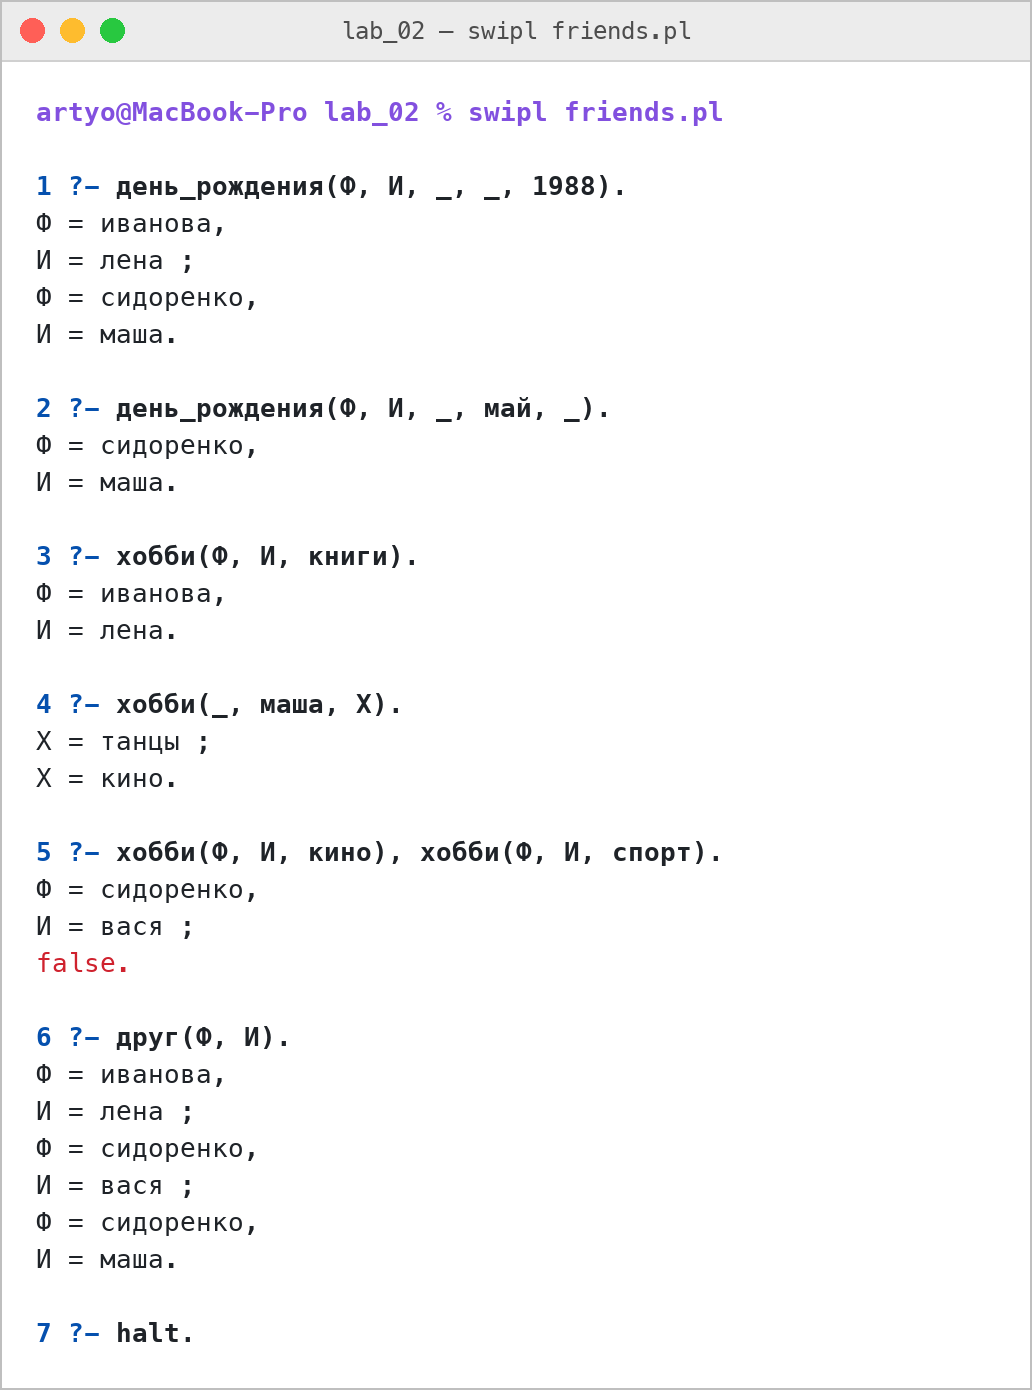
\includegraphics[width=0.62\textwidth]{fig05_friends_queries.png}
\caption{Ответы на вопросы варианта~3 в интерактивном режиме}
\label{fig:friends-queries}
\end{figure}

Те же ответы выводит предикат \code{ответы/0}; запрос с \code{findall/3} собирает список друзей одним значением (рисунок~\ref{fig:friends-answers}).

\begin{figure}[H]
\centering
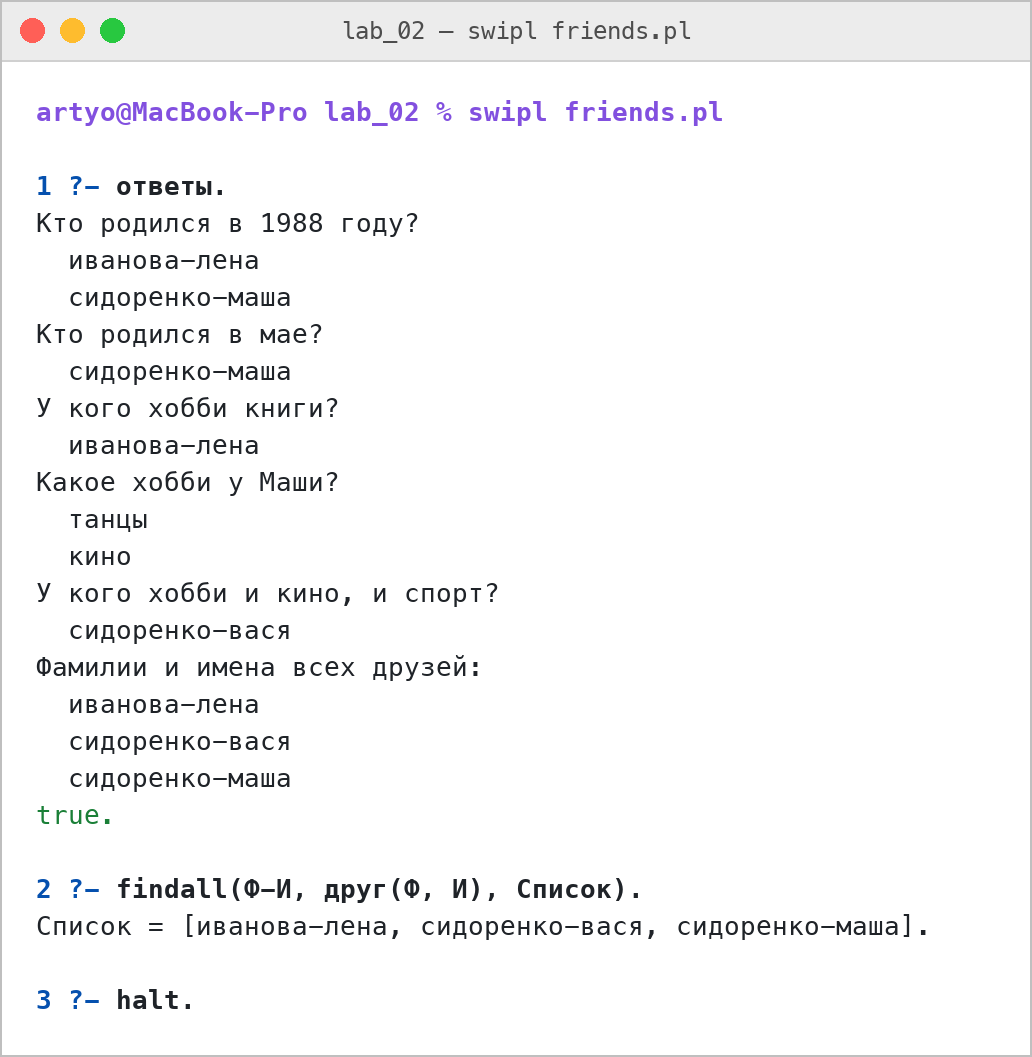
\includegraphics[width=0.62\textwidth]{fig06_friends_answers.png}
\caption{Результат работы предиката \code{ответы/0} и список друзей одним термом}
\label{fig:friends-answers}
\end{figure}

\subsection{Задание 4: логическая задача <<Спортсмены>> (вариант 3)}

\textbf{Условие.} Тонни, Майкл и Джон~--- спортсмены. Один из них боксёр, другой футболист, третий пловец. Один любит снег, другой~--- дождь, третий~--- солнечную погоду. Тот, кто любит солнечную погоду,~--- не боксёр. Тонни не любит снег. Майкл не любит солнечную погоду. Футболист любит снег. Тонни не пловец. Определить, у кого какая любимая погода и кто каким спортом занимается.

\textbf{Формализация.} Каждый спортсмен описывается термом \code{человек(Имя, Спорт, Погода)}. Три спортсмена образуют список, в котором виды спорта и виды погоды~--- перестановки трёх возможных значений: так выполняется условие <<один~--- боксёр, другой~--- футболист, третий~--- пловец>> (и то же для погоды). Остальные условия записаны как ограничения (таблица~\ref{tab:constraints}).

\begin{longtable}{@{}p{0.05\textwidth}p{0.36\textwidth}p{0.5\textwidth}@{}}
\caption{Запись условий задачи на Прологе}\label{tab:constraints}\\
\toprule
№ & Условие & Цель \\
\midrule
\endfirsthead
\toprule
№ & Условие & Цель \\
\midrule
\endhead
1 & Любящий солнце не боксёр & \code{\textbackslash+ member(человек(\_, боксёр, солнце), Люди)} \\
2 & Тонни не любит снег & \code{\textbackslash+ member(человек(тонни, \_, снег), Люди)} \\
3 & Майкл не любит солнце & \code{\textbackslash+ member(человек(майкл, \_, солнце), Люди)} \\
4 & Футболист любит снег & \code{member(человек(\_, футболист, снег), Люди)} \\
5 & Тонни не пловец & \code{\textbackslash+ member(человек(тонни, пловец, \_), Люди)} \\
\bottomrule
\end{longtable}

\textbf{Решение.} Программа \code{lab\_02/sportsmen.pl} использует метод <<образовать и проверить>>: \code{решение/1} перебирает $3!\cdot 3! = 36$ вариантов распределения значений, а \code{ограничения/1} отбрасывает не удовлетворяющие условиям. Предикат \code{решить/0} находит все решения, сообщает их число и печатает.

\VerbatimInput{../sportsmen.pl}

\textbf{Результат} показан на рисунке~\ref{fig:sportsmen}. Найдено ровно одно решение, значит условия определяют ответ однозначно:

\begin{itemize}
\item Тонни~--- боксёр, любит дождь;
\item Майкл~--- футболист, любит снег;
\item Джон~--- пловец, любит солнечную погоду.
\end{itemize}

\begin{figure}[H]
\centering
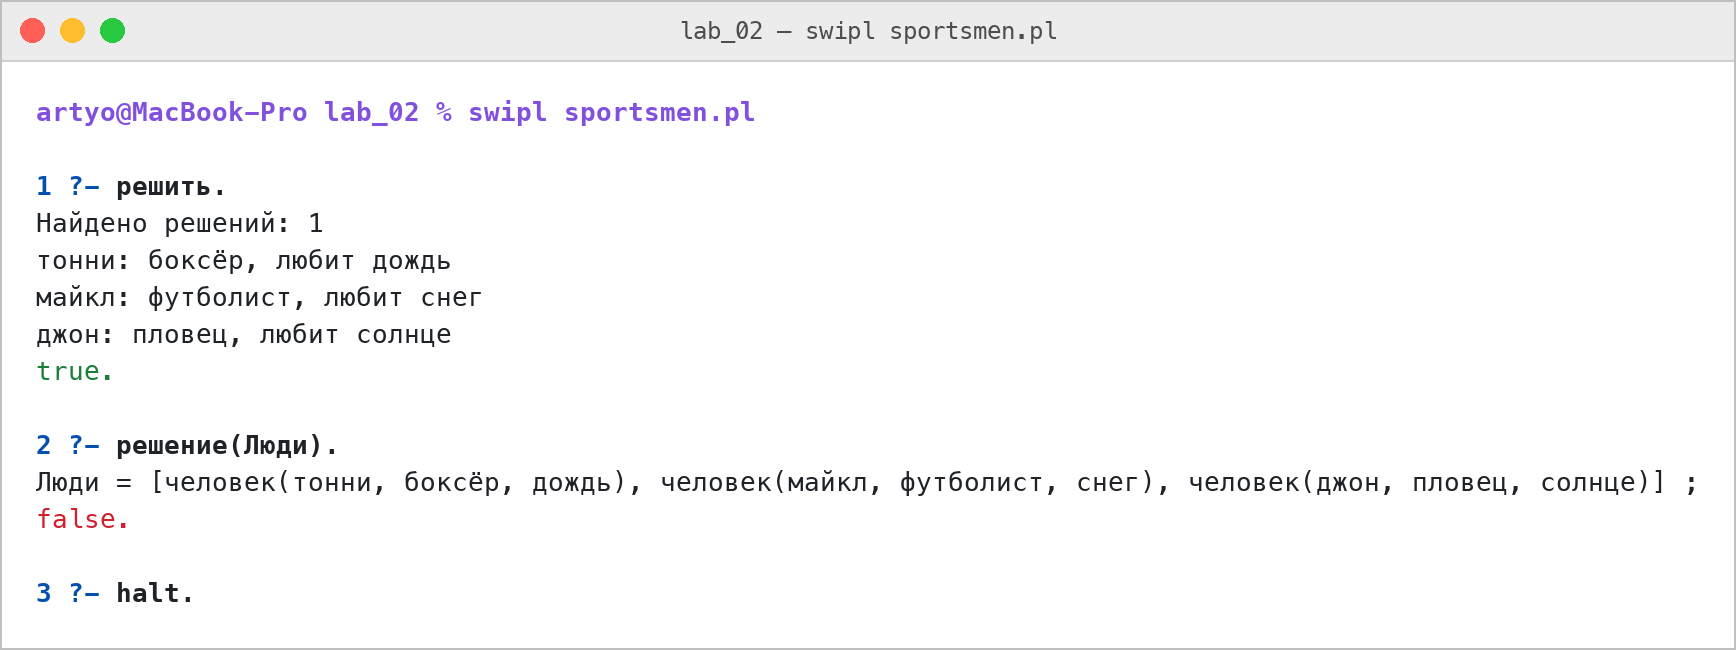
\includegraphics[width=\textwidth]{fig07_sportsmen.png}
\caption{Решение логической задачи: результат \code{решить/0} и запрос \code{решение(Люди)}}
\label{fig:sportsmen}
\end{figure}

\textbf{Проверка рассуждением.} Футболист любит снег (условие~4), а Тонни снег не любит (2) и не пловец (5), поэтому Тонни~--- не футболист и не пловец, то есть боксёр. Боксёр не любит солнце (1) и снег (снег любит футболист), значит Тонни любит дождь. Майкл не любит солнце (3) и дождь уже занят, поэтому Майкл любит снег и является футболистом, а Джон остаётся пловцом, любящим солнце. Ответ совпадает с результатом программы.

\section{Анализ результатов}

\begin{enumerate}
\item \textbf{Динамическая база.} Факты, добавленные \code{assertz/1}, существуют только в памяти текущего сеанса и исчезают при его завершении; \code{listing/1} выводит их с пометкой \code{:- dynamic}. Статические факты \code{friends.pl} изменять в ходе работы нельзя.
\item \textbf{Транзитивность и циклы.} Рекурсивное правило \code{greater/2} завершается только на ациклических данных, поэтому контроль противоречий вынесен в момент добавления факта. Это дешевле, чем защищать от зацикливания каждый запрос (например, табличным выполнением).
\item \textbf{Частичный порядок.} Введённых отношений часто недостаточно для полного упорядочения. Самый большой объект~--- тот, для которого нет большего, но таких объектов может быть несколько; вывод всех максимальных элементов честнее выбора одного произвольного. Пример из задания именно такой: ответ об одном <<самом большом>> объекте зависит от того, достаточно ли введённых условий.
\item \textbf{Остаточные точки выбора.} Ответ \code{true ;} \code{false.} на запросах \code{greater(\ldots)}, \code{largest(X)} и \code{решение(Люди)} означает, что после найденного решения у системы остались непроверенные альтернативы, но других решений нет. Для \code{решение/1} это следствие метода <<образовать и проверить>>: после первого удачного распределения перебор продолжается и подтверждает единственность решения.
\item \textbf{Отрицание как неуспех.} Правила \code{largest/1}, \code{smallest/1} и ограничения задачи используют \code{\textbackslash+}. Оно корректно только при полностью определённых аргументах: в \code{largest/1} цель \code{object(X)} стоит перед \code{\textbackslash+}, чтобы \code{X} был связан к моменту проверки.
\item \textbf{Кириллица.} SWI-Prolog 10 читает исходные файлы в UTF-8; атомы и предикаты можно писать кириллицей, переменная начинается с заглавной буквы (\code{Ф}, \code{Люди}). При печати через \code{format/2} и в top-level атомы выводятся без кавычек.
\end{enumerate}

\section{Выводы}

В ходе работы в SWI-Prolog 10.0.2 созданы три программы. Для задания~2 реализована динамическая база фактов, пополняемая вводом с консоли до символа остановки, с проверкой противоречий и правилами для поиска наибольшего и наименьшего объектов; на примере из задания получены самый маленький объект (вишня) и два несравнимых максимальных (яблоко и дуриан), а после добавления недостающего условия~--- единственный наибольший (дуриан). Для задания~3 записана база знаний <<Друзья>> варианта~3 и получены ответы на все шесть вопросов. Для задания~4 логическая задача решена методом <<образовать и проверить>>; найдено единственное решение, совпавшее с ручным рассуждением.

В процессе освоены \code{assertz/retractall}, объявление \code{dynamic}, построчный ввод, транзитивные правила, отрицание как неуспех, сбор решений \code{findall/3} и перестановки \code{permutation/2}. Серьёзных трудностей не возникло; единственное, что потребовало решения,~--- возможное зацикливание \code{greater/2} на противоречивых данных, устранённое проверкой при добавлении факта.

\newpage
\sectioncenter{Приложение А. Контрольные вопросы для Moodle}

Ниже приведены 30 контрольных вопросов в форме, удобной для визуальной проверки. Исходный банк вопросов для загрузки в Moodle хранится в файле \code{moodle\_questions\_gift.txt} в формате GIFT.

\small
\begin{enumerate}[label=\textbf{\arabic*.}, leftmargin=0pt, itemsep=1.2em]
\item Для чего служит директива :- dynamic bigger/2. в начале программы?
\begin{itemize}[label=$\square$, leftmargin=1.5cm, itemsep=0.2em, topsep=0.3em]
\item Включает трассировку предиката bigger/2
\item Объявляет, что клаузы bigger/2 можно добавлять и удалять во время выполнения
\item Запрещает изменять факты bigger/2 после загрузки файла
\item Делает предикат bigger/2 видимым из других файлов
\end{itemize}
{\small\textit{Правильный ответ: Объявляет, что клаузы bigger/2 можно добавлять и удалять во время выполнения.}}

\item Чем assertz/1 отличается от asserta/1?
\begin{itemize}[label=$\square$, leftmargin=1.5cm, itemsep=0.2em, topsep=0.3em]
\item assertz удаляет клаузу, а asserta добавляет
\item assertz добавляет клаузу в конец предиката, asserta — в начало
\item assertz работает только с фактами, asserta — только с правилами
\item Ничем, это синонимы
\end{itemize}
{\small\textit{Правильный ответ: assertz добавляет клаузу в конец предиката, asserta — в начало.}}

\item Что делает вызов retractall(bigger(\_, \_))?
\begin{itemize}[label=$\square$, leftmargin=1.5cm, itemsep=0.2em, topsep=0.3em]
\item Удаляет только первый факт bigger/2
\item Удаляет все клаузы bigger/2, при этом сам предикат остаётся определённым
\item Выводит все факты bigger/2 на экран
\item Завершает работу интерпретатора
\end{itemize}
{\small\textit{Правильный ответ: Удаляет все клаузы bigger/2, при этом сам предикат остаётся определённым.}}

\item Чем retract/1 отличается от retractall/1?
\begin{itemize}[label=$\square$, leftmargin=1.5cm, itemsep=0.2em, topsep=0.3em]
\item retract удаляет первую подходящую клаузу и при возврате — следующие, retractall удаляет все подходящие за один вызов
\item retract удаляет предикат целиком, retractall — только факты
\item retractall можно применять только к статическим предикатам
\item Ничем
\end{itemize}
{\small\textit{Правильный ответ: retract удаляет первую подходящую клаузу и при возврате — следующие, retractall удаляет все подходящие за один вызов.}}

\item Что вернёт read\_line\_to\_string(user\_input, L) при достижении конца ввода (Ctrl+D)?
\begin{itemize}[label=$\square$, leftmargin=1.5cm, itemsep=0.2em, topsep=0.3em]
\item Пустую строку ""
\item Атом halt
\item Ошибку синтаксиса
\item Атом end\_of\_file
\end{itemize}
{\small\textit{Правильный ответ: Атом end\_of\_file.}}

\item Каков результат split\_string("яблоко > слива", " ", "", P)?
\begin{itemize}[label=$\square$, leftmargin=1.5cm, itemsep=0.2em, topsep=0.3em]
\item P = "яблоко > слива"
\item P = [яблоко, >, слива]
\item P = ["яблоко", ">", "слива"]
\item false.
\end{itemize}
{\small\textit{Правильный ответ: P = ["яблоко", ">", "слива"].}}

\item Для чего в программе используется normalize\_space(string(Clean), Line)?
\begin{itemize}[label=$\square$, leftmargin=1.5cm, itemsep=0.2em, topsep=0.3em]
\item Переводит строку в нижний регистр
\item Убирает лишние пробелы в начале, конце и между словами
\item Разбивает строку на слова
\item Преобразует строку в число
\end{itemize}
{\small\textit{Правильный ответ: Убирает лишние пробелы в начале, конце и между словами.}}

\item Зачем после format("ввод: ") вызывают flush\_output?
\begin{itemize}[label=$\square$, leftmargin=1.5cm, itemsep=0.2em, topsep=0.3em]
\item Чтобы очистить экран терминала
\item Чтобы закрыть поток вывода
\item Чтобы приглашение без перевода строки немедленно появилось на экране до чтения ввода
\item Чтобы удалить введённые ранее данные
\end{itemize}
{\small\textit{Правильный ответ: Чтобы приглашение без перевода строки немедленно появилось на экране до чтения ввода.}}

\item Что делает вызов prompt(Old, '') перед чтением строк из user\_input?
\begin{itemize}[label=$\square$, leftmargin=1.5cm, itemsep=0.2em, topsep=0.3em]
\item Запоминает прежнее приглашение в Old и заменяет его пустым, чтобы не выводилось «|: »
\item Запрещает вводить пустые строки
\item Очищает буфер ввода
\item Загружает файл с пустым именем
\end{itemize}
{\small\textit{Правильный ответ: Запоминает прежнее приглашение в Old и заменяет его пустым, чтобы не выводилось «|: ».}}

\item Зачем у правила greater/2 две клаузы?
\begin{itemize}[label=$\square$, leftmargin=1.5cm, itemsep=0.2em, topsep=0.3em]
\item Вторая клауза нужна для обработки ошибок
\item Первая — базовый случай (прямой факт bigger), вторая — рекурсивный шаг по цепочке отношений
\item Первая работает с числами, вторая — с атомами
\item Две клаузы нужны только для ускорения поиска
\end{itemize}
{\small\textit{Правильный ответ: Первая — базовый случай (прямой факт bigger), вторая — рекурсивный шаг по цепочке отношений.}}

\item Что произошло бы с greater/2 при цикле в фактах (a больше b, b больше a)?
\begin{itemize}[label=$\square$, leftmargin=1.5cm, itemsep=0.2em, topsep=0.3em]
\item Запрос вернул бы false
\item Интерпретатор отказался бы загружать факты
\item Рекурсия не имела бы конца и привела бы к переполнению стека
\item Результат зависел бы только от порядка ввода
\end{itemize}
{\small\textit{Правильный ответ: Рекурсия не имела бы конца и привела бы к переполнению стека.}}

\item Какую роль выполняет клауза add\_relation(X, Y) :- greater(Y, X), !, ...?
\begin{itemize}[label=$\square$, leftmargin=1.5cm, itemsep=0.2em, topsep=0.3em]
\item Добавляет новый факт в базу
\item Обнаруживает противоречие: Y уже больше X, и отклоняет новый факт
\item Удаляет старые факты
\item Сортирует объекты по размеру
\end{itemize}
{\small\textit{Правильный ответ: Обнаруживает противоречие: Y уже больше X, и отклоняет новый факт.}}

\item Как читается правило largest(X) :- object(X), \textbackslash{}+ bigger(\_, X).?
\begin{itemize}[label=$\square$, leftmargin=1.5cm, itemsep=0.2em, topsep=0.3em]
\item X больше любого объекта
\item X — объект, для которого не найдётся ни одного объекта, больший X
\item X — объект, который больше самого себя
\item X — любой объект, имеющий хотя бы один факт bigger
\end{itemize}
{\small\textit{Правильный ответ: X — объект, для которого не найдётся ни одного объекта, больший X.}}

\item Что означает оператор \textbackslash{}+ в Прологе?
\begin{itemize}[label=$\square$, leftmargin=1.5cm, itemsep=0.2em, topsep=0.3em]
\item Арифметическое сложение
\item Логическое отрицание в смысле математической логики
\item Отрицание как неуспех: цель \textbackslash{}+ G успешна, если доказать G не удаётся
\item Объединение двух списков
\end{itemize}
{\small\textit{Правильный ответ: Отрицание как неуспех: цель \textbackslash{}+ G успешна, если доказать G не удаётся.}}

\item Что делает предикат findall(X, largest(X), L)?
\begin{itemize}[label=$\square$, leftmargin=1.5cm, itemsep=0.2em, topsep=0.3em]
\item Находит первое решение и останавливается
\item Удаляет все решения largest/1 из базы
\item Собирает в список L значения X по всем решениям largest(X)
\item Проверяет, что largest/1 определён
\end{itemize}
{\small\textit{Правильный ответ: Собирает в список L значения X по всем решениям largest(X).}}

\item Почему для примера из задания (яблоко, слива, авокадо, папайя, дуриан, вишня) нет единого самого большого объекта?
\begin{itemize}[label=$\square$, leftmargin=1.5cm, itemsep=0.2em, topsep=0.3em]
\item Потому что вводились не все объекты
\item Потому что дуриан меньше папайи
\item Яблоко и дуриан не связаны цепочкой отношений, и ни один из них не доказуемо больше другого
\item Потому что в Прологе нельзя сравнивать более пяти объектов
\end{itemize}
{\small\textit{Правильный ответ: Яблоко и дуриан не связаны цепочкой отношений, и ни один из них не доказуемо больше другого.}}

\item Какой самый маленький объект в примере с фруктами из задания?
\begin{itemize}[label=$\square$, leftmargin=1.5cm, itemsep=0.2em, topsep=0.3em]
\item слива
\item авокадо
\item вишня
\item яблоко
\end{itemize}
{\small\textit{Правильный ответ: вишня.}}

\item Для чего служит вызов aggregate\_all(count, bigger(\_, \_), M)?
\begin{itemize}[label=$\square$, leftmargin=1.5cm, itemsep=0.2em, topsep=0.3em]
\item Суммирует значения аргументов bigger/2
\item Подсчитывает число решений цели, то есть число фактов bigger/2
\item Удаляет дубликаты фактов
\item Сортирует факты по возрастанию
\end{itemize}
{\small\textit{Правильный ответ: Подсчитывает число решений цели, то есть число фактов bigger/2.}}

\item Какой арности предикат день\_рождения(иванова, лена, 12, июнь, 1988)?
\begin{itemize}[label=$\square$, leftmargin=1.5cm, itemsep=0.2em, topsep=0.3em]
\item 3
\item 4
\item 5
\item 6
\end{itemize}
{\small\textit{Правильный ответ: 5.}}

\item Какие люди вернёт запрос \texttt{?-} день\_рождения(Ф, И, \_, \_, 1988).?
\begin{itemize}[label=$\square$, leftmargin=1.5cm, itemsep=0.2em, topsep=0.3em]
\item Только Лену Иванову
\item Только Васю Сидоренко
\item Лену Иванову и Машу Сидоренко
\item Всех троих друзей
\end{itemize}
{\small\textit{Правильный ответ: Лену Иванову и Машу Сидоренко.}}

\item Что означает символ \_ в запросе \texttt{?-} день\_рождения(Ф, И, \_, май, \_).?
\begin{itemize}[label=$\square$, leftmargin=1.5cm, itemsep=0.2em, topsep=0.3em]
\item Пустое значение, которое обязательно нужно подставить
\item Имя предиката
\item Анонимная переменная: значение на этой позиции не важно и не запоминается
\item Знак вычитания
\end{itemize}
{\small\textit{Правильный ответ: Анонимная переменная: значение на этой позиции не важно и не запоминается.}}

\item Сколько решений даст запрос \texttt{?-} хобби(\_, маша, Х).?
\begin{itemize}[label=$\square$, leftmargin=1.5cm, itemsep=0.2em, topsep=0.3em]
\item 0
\item 1
\item 2
\item 3
\end{itemize}
{\small\textit{Правильный ответ: 2.}}

\item Почему запрос \texttt{?-} хобби(Ф, И, кино), хобби(Ф, И, спорт). находит именно Васю?
\begin{itemize}[label=$\square$, leftmargin=1.5cm, itemsep=0.2em, topsep=0.3em]
\item Потому что Вася родился раньше всех
\item Одни и те же переменные Ф и И в обеих целях требуют, чтобы оба хобби принадлежали одному человеку
\item Потому что запятая означает «или»
\item Потому что Вася — единственный друг в базе
\end{itemize}
{\small\textit{Правильный ответ: Одни и те же переменные Ф и И в обеих целях требуют, чтобы оба хобби принадлежали одному человеку.}}

\item Какое имя в SWI-Prolog является переменной?
\begin{itemize}[label=$\square$, leftmargin=1.5cm, itemsep=0.2em, topsep=0.3em]
\item иванова
\item 'Лена'
\item Ф
\item маша
\end{itemize}
{\small\textit{Правильный ответ: Ф.}}

\item Как называется метод решения логической задачи в программе sportsmen.pl?
\begin{itemize}[label=$\square$, leftmargin=1.5cm, itemsep=0.2em, topsep=0.3em]
\item Динамическое программирование
\item Метод наименьших квадратов
\item Жадный алгоритм
\item Образовать и проверить (generate and test)
\end{itemize}
{\small\textit{Правильный ответ: Образовать и проверить (generate and test).}}

\item Сколько различных результатов даёт запрос \texttt{?-} findall(P, permutation([a, b, c], P), L), length(L, N).?
\begin{itemize}[label=$\square$, leftmargin=1.5cm, itemsep=0.2em, topsep=0.3em]
\item 3
\item 6
\item 9
\item 27
\end{itemize}
{\small\textit{Правильный ответ: 6.}}

\item Зачем для видов спорта и для погоды используют permutation/2, а не независимый выбор значений?
\begin{itemize}[label=$\square$, leftmargin=1.5cm, itemsep=0.2em, topsep=0.3em]
\item Для ускорения работы интерпретатора
\item Перестановка гарантирует, что значения признака у троих спортсменов различны и все использованы
\item Чтобы получить значения в алфавитном порядке
\item Это требуется синтаксисом SWI-Prolog
\end{itemize}
{\small\textit{Правильный ответ: Перестановка гарантирует, что значения признака у троих спортсменов различны и все использованы.}}

\item Какое условие задачи выражает цель \textbackslash{}+ member(человек(\_, боксёр, солнце), Люди)?
\begin{itemize}[label=$\square$, leftmargin=1.5cm, itemsep=0.2em, topsep=0.3em]
\item Боксёр любит только солнечную погоду
\item Тот, кто любит солнечную погоду, не боксёр
\item Среди спортсменов нет людей
\item Все любят солнечную погоду
\end{itemize}
{\small\textit{Правильный ответ: Тот, кто любит солнечную погоду, не боксёр.}}

\item Кем является Тонни согласно найденному решению?
\begin{itemize}[label=$\square$, leftmargin=1.5cm, itemsep=0.2em, topsep=0.3em]
\item Футболистом, любит снег
\item Пловцом, любит солнце
\item Футболистом, любит дождь
\item Боксёром, любит дождь
\end{itemize}
{\small\textit{Правильный ответ: Боксёром, любит дождь.}}

\item Что подтверждает результат «Найдено решений: 1» для логической задачи?
\begin{itemize}[label=$\square$, leftmargin=1.5cm, itemsep=0.2em, topsep=0.3em]
\item Что программа завершилась без ошибок и это всё
\item Что условия задачи определяют ответ однозначно
\item Что в задаче нет ограничений
\item Что программа проверила только один вариант
\end{itemize}
{\small\textit{Правильный ответ: Что условия задачи определяют ответ однозначно.}}
\end{enumerate}
\normalsize


\end{document}
